\documentclass[a4]{article}
\usepackage{graphicx} % Required for inserting images
\usepackage{booktabs}
\usepackage{pdflscape}

%\documentclass[12pt]{article}
\usepackage[utf8]{inputenc}
\usepackage{fourier} 
\usepackage{array}
\usepackage{makecell}


\usepackage[margin=0.5in]{geometry}

\renewcommand\theadalign{bc}
\renewcommand\theadfont{\bfseries}
\renewcommand\theadgape{\Gape[4pt]}
\renewcommand\cellgape{\Gape[4pt]}

\title{Batch 1 Sample Preparation Data Tables \& Figures \\ Congruent melting RHEA research project \\ ---\\Tasan Group - MIT DMSE \\ Pham Group - imperial Materials \\}
\author{Sigurd Bjerkhaug}
\date{October 2023}

\begin{document}

\maketitle

\newpage




\section{Prepared samples}

\begin{table}[h]
    \centering
    \caption{Alloys weighed out}
    \begin{tabular}{llllll}
\toprule
\thead{Shortcode} &          \thead{Composition \\ At\%} &                     \thead{Composition \\ Wt\%} & \thead{Total target weight \\ sample} &                                                     \thead{Target weight \\ per element} &                                               \thead{Measure weight \\ per element} \\
\midrule
             B1-1 &        $Ti_{38}V_{15}Nb_{23}Hf_{24}$ &           $Ti_{20.2}V_{8.49}Nb_{23.7}Hf_{47.6}$ &                                10.0 g &                \makecell[l]{ Ti : 2.02 g \\ V : 0.85 g \\ Nb : 2.37 g \\ Hf : 4.76 g \\} &               \makecell[l]{ Ti : 2.09 g\\ V : 0.83 g\\ Nb : 2.28 g\\ Hf : 4.74 g\\} \\
             B1-2 &        $Ti_{25}V_{25}Nb_{25}Hf_{25}$ &           $Ti_{12.9}V_{13.8}Nb_{25.1}Hf_{48.2}$ &                                10.0 g &                \makecell[l]{ Ti : 1.29 g \\ V : 1.38 g \\ Nb : 2.51 g \\ Hf : 4.82 g \\} &               \makecell[l]{ Ti : 1.32 g\\ V : 1.40 g\\ Nb : 1.46 g\\ Hf : 4.80 g\\} \\
             B1-3 & $Ti_{20}V_{20}Nb_{20}Hf_{20}Si_{20}$ &  $Ti_{12.0}V_{12.8}Nb_{23.3}Hf_{44.8}Si_{7.05}$ &                                10.0 g & \makecell[l]{ Ti : 1.20 g \\ V : 1.28 g \\ Nb : 2.33 g \\ Hf : 4.48 g \\ Si : 0.71 g \\} & \makecell[l]{ Ti : 1.21 g\\ V : 1.28 g\\ Nb : 2.29 g\\ Hf : 4.52 g\\ Si : 1.15 g\\} \\
             B1-4 &  $Ti_{38}V_{15}Nb_{23}Hf_{23}Si_{1}$ & $Ti_{20.5}V_{8.63}Nb_{24.1}Hf_{46.4}Si_{0.317}$ &                                10.0 g & \makecell[l]{ Ti : 2.05 g \\ V : 0.86 g \\ Nb : 2.41 g \\ Hf : 4.64 g \\ Si : 0.03 g \\} & \makecell[l]{ Ti : 2.09 g\\ V : 0.87 g\\ Nb : 2.50 g\\ Hf : 4.67 g\\ Si : 0.92 g\\} \\
             B1-5 & $Ti_{20}V_{20}Nb_{20}Hf_{20}Cr_{20}$ &  $Ti_{11.3}V_{12.1}Nb_{22.0}Hf_{42.3}Cr_{12.3}$ &                                10.0 g & \makecell[l]{ Ti : 1.13 g \\ V : 1.21 g \\ Nb : 2.20 g \\ Hf : 4.23 g \\ Cr : 1.23 g \\} & \makecell[l]{ Ti : 1.10 g\\ V : 1.21 g\\ Nb : 2.09 g\\ Hf : 4.13 g\\ Cr : 1.91 g\\} \\
\bottomrule
\end{tabular}

    \label{tab:Batch1 mesured}
\end{table}

from the target composition we would expect properties as tabulated in table
\begin{table}[h]
    \centering
    \caption{Batch 1 alloy estimated properties}
    \begin{tabular}{lllllll}
\toprule
\thead{index} &          \thead{Composition \\ At\%} & \thead{Price \\ USD} & \thead{Density \\ g cm$^{-3}$} & \thead{T$_{Liquidus}$ \\ C$^{o}$} & \thead{T$_{Solidus}$ \\ C$^{o}$} & \thead{ΔT$_{Liquidus - Solidus}$ \\ C$^{o}$} \\
\midrule
         B1-1 &        $Ti_{38}V_{15}Nb_{23}Hf_{24}$ &              1313.28 &                           7.79 &                              1750 &                             1650 &                                         1650 \\
         B1-2 &        $Ti_{25}V_{25}Nb_{25}Hf_{25}$ &              1370.50 &                           8.12 &                              1727 &                             1590 &                                         1590 \\
         B1-3 & $Ti_{20}V_{20}Nb_{20}Hf_{20}Si_{20}$ &              1096.70 &                           6.96 &                              1715 &                             1279 &                                         1279 \\
         B1-4 &  $Ti_{38}V_{15}Nb_{23}Hf_{23}Si_{1}$ &              1259.30 &                           7.68 &                              1733 &                             1175 &                                         1175 \\
         B1-5 & $Ti_{20}V_{20}Nb_{20}Hf_{20}Cr_{20}$ &              1097.80 &                           7.94 &                              1528 &                             1361 &                                         1361 \\
\bottomrule
\end{tabular}

    \label{tab:Batch1 mesured}
\end{table}

\begin{table}[h]
    \centering
    \caption{Alloy target vs experimental}
    \begin{tabular}{llll}
\toprule
\thead{shortcode} &   \thead{Target Composition \\ At\%} &           \thead{Measured Composition \\ At\%} &        \thead{deviation of composition \\ At\%} \\
\midrule
        \\ B1-1 \ &        $Ti_{38}V_{15}Nb_{23}Hf_{24}$ &          $Ti_{39.3}V_{14.7}Nb_{22.1}Hf_{23.9}$ &      $Ti_{-1.32}V_{0.329}Nb_{0.902}Hf_{0.0869}$ \\
        \\ B1-2 \ &        $Ti_{25}V_{25}Nb_{25}Hf_{25}$ &          $Ti_{28.2}V_{28.1}Nb_{16.1}Hf_{27.5}$ &        $Ti_{-3.24}V_{-3.14}Nb_{8.91}Hf_{-2.54}$ \\
        \\ B1-3 \ & $Ti_{20}V_{20}Nb_{20}Hf_{20}Si_{20}$ & $Ti_{17.9}V_{17.8}Nb_{17.4}Hf_{17.9}Si_{29.0}$ & $Ti_{2.11}V_{2.22}Nb_{2.56}Hf_{2.08}Si_{-8.97}$ \\
        \\ B1-4 \ &  $Ti_{38}V_{15}Nb_{23}Hf_{23}Si_{1}$ & $Ti_{29.8}V_{11.7}Nb_{18.4}Hf_{17.9}Si_{22.3}$ & $Ti_{8.21}V_{3.35}Nb_{4.64}Hf_{5.15}Si_{-21.3}$ \\
        \\ B1-5 \ & $Ti_{20}V_{20}Nb_{20}Hf_{20}Cr_{20}$ & $Ti_{17.8}V_{18.4}Nb_{17.4}Hf_{17.9}Cr_{28.5}$ &   $Ti_{2.2}V_{1.6}Nb_{2.57}Hf_{2.08}Cr_{-8.45}$ \\
\bottomrule
\end{tabular}

    \label{tab:Batch1 mesured}
\end{table}

%\begin{table}[h]
%    \centering
%    \caption{Alloy target vs experimental}
%    \begin{tabular}{cccc}
\toprule
{} &    Producer &   Purity & Morphology \\
\midrule
Ti &  Alfa Aesar &    99.98 &    Pellets \\
V  &  Alfa Aesar &     99.7 &  Platelets \\
Nb &  Alfa Aesar &    99.95 &    Pellets \\
Hf &         BTC &     99.9 &      Swarf \\
Si &  Alfa Aesar &  99.9999 &      Lumps \\
Cr &  Alfa Aesar &    99.95 &      Cubes \\
\bottomrule
\end{tabular}

%    \label{tab:Batch1 mesured}
%\end{table}

\begin{figure}
    \centering
    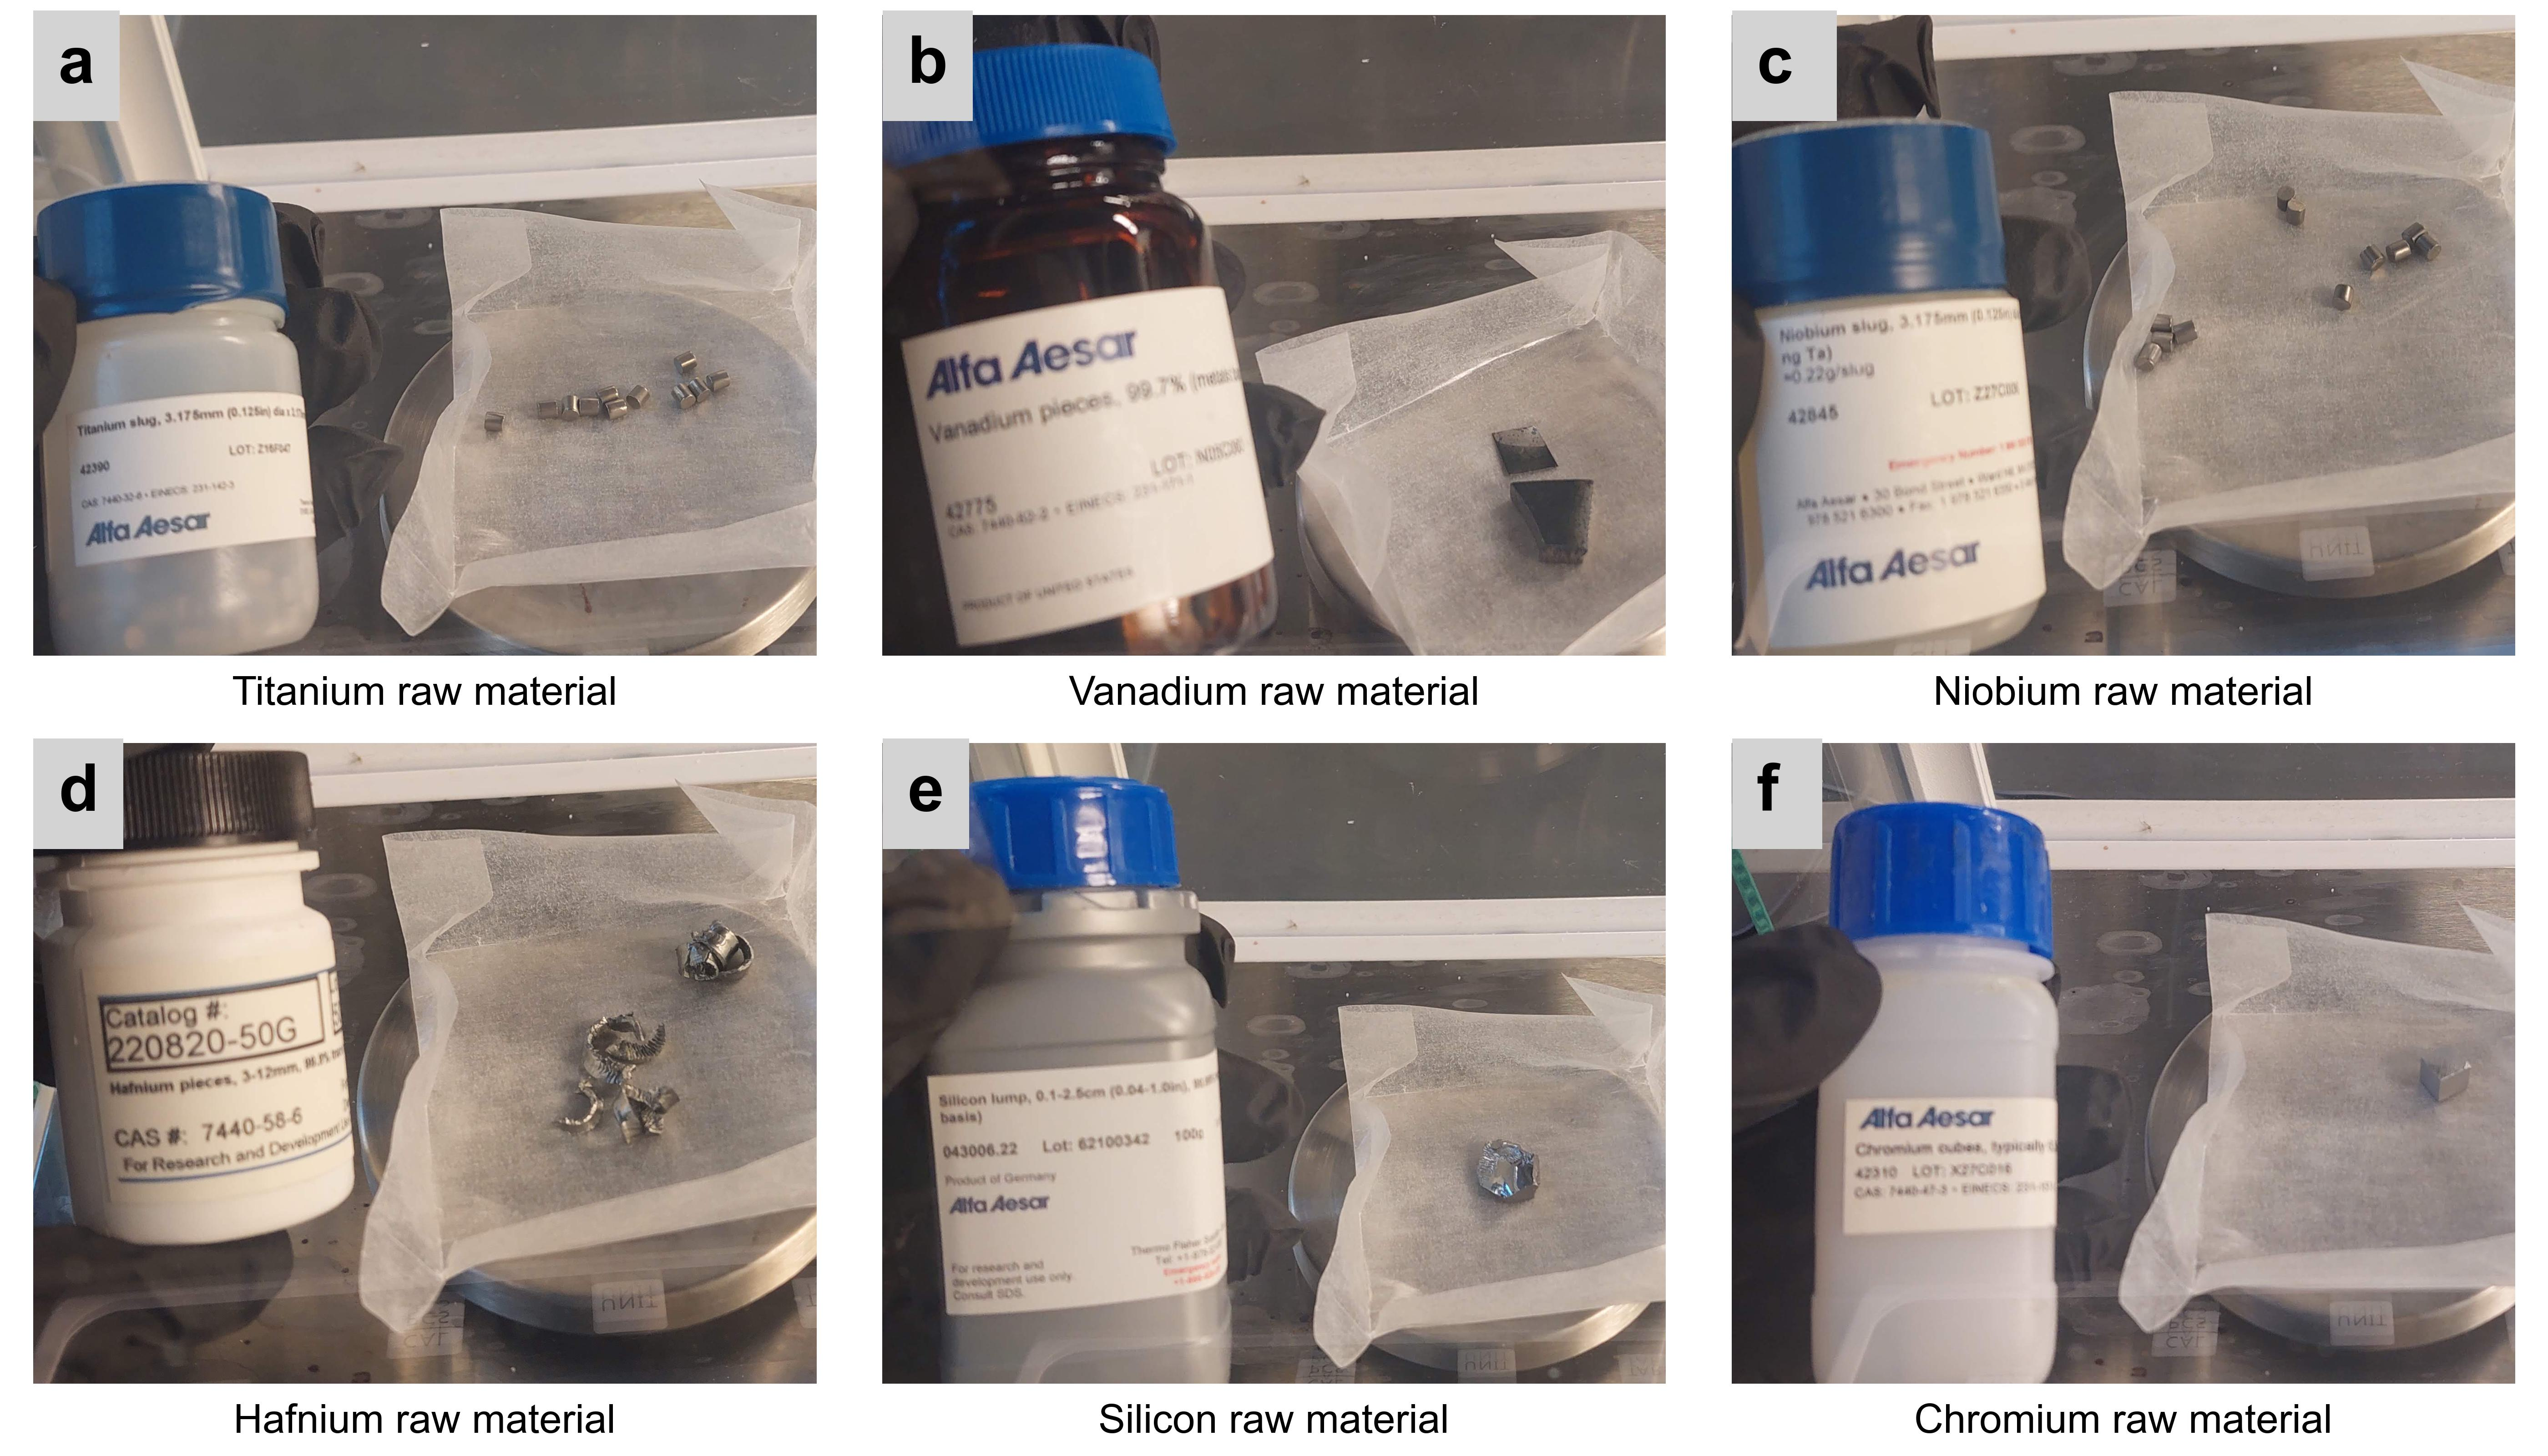
\includegraphics{batch 1 raw materials.jpg}
    \caption{Raw materials used}
    \label{fig:raw-material info}
\end{figure}

\begin{figure}
    \centering
    \includegraphics{Batch 1_Arc melting figure.png}
    \caption{Caption}
    \label{fig:arc-melted samples}
\end{figure}

\begin{tabular}{ccccc}
\toprule
{} &    Producer &   Purity & Morphology & total use batch 1 \\
\midrule
Ti &  Alfa Aesar &    99.98 &    Pellets &            9.81  g \\
V  &  Alfa Aesar &     99.7 &  Platelets &            10.0 g \\
Nb &  Alfa Aesar &    99.95 &    Pellets &           12.91 g \\
Hf &         BTC &     99.9 &      Swarf &           27.24 g \\
Si &  Alfa Aesar &  99.9999 &      Lumps &            2.07 g \\
Cr &  Alfa Aesar &    99.95 &      Cubes &            1.91 g \\
\bottomrule
\end{tabular}

\end{document}
